La librairie Keras est une interface Python/TensorFlow\cite{tf} permetant de travailler avec des réseaux de neurones.
Ici, on ne s'attardera que sur les fonctionnalitées principales,
a savoir la création d'un réseau simple,
la regression par \sgd\ et l'évaluation des performances.


Voici un exemple de réseau de neurone assez simple
qui vas essayer de deviner l'application linéaire suivante : $f(X) = 0.2x_1 + 0.8x_2$.

\begin{figure}[H]
    \center
    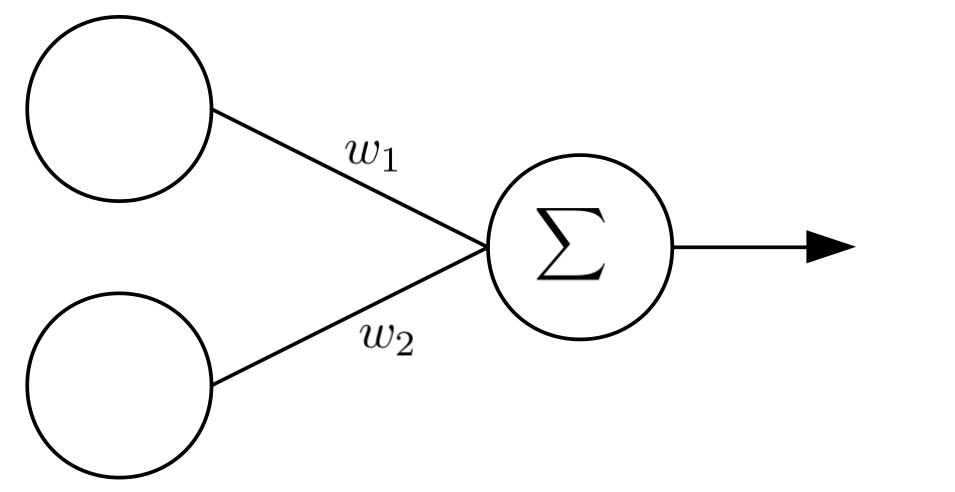
\includegraphics[height=\petit]{pict/net2.png}
	\caption{Réseau simple}
	\label{fig:net2}
\end{figure}
\vspace{-12pt}


Pour créer ce réseau et lui faire apprendre la fonction precedement citée,
le code suivant est nescessaire :
\lstinputlisting[language=Python]{code/reseau1.py}


En executant ce code, on obtient:
\begin{lstlisting}
w0 : 0.19988934695720673
w1 : 0.8001111745834351
\end{lstlisting}
On peut donc bien voir que le réseau de neurones fonctionne et
réussit à apprendre des fonctions avec plusieurs paramètres.
Il est cependant assez embetant de toujours devoir faire appel a toutes ces fonctions.
Une librairie à alors été codée afin de simplifier son utilisation.
Elle pourra être appelée avec de nombreux paramtres qui seront abordés dans les parties suivantes.\\


Pour tester la robustesse de cet apprentissage, une fonction avec perturbations à été étudiée :
Une fonction simple à été générée comme precedement, il y a été ajouté une perturbation random equiprobable
entre $ - err$ et $err$.
L’erreur d’apprentissage en fonction de la valeur de $err$ à alors été étudiée.\\

\paragraph{Un probleme se pose :}
Prennons la formule (\ref{eq:choquet}) avec, par exemple, $n = 2$ :
\begin{align*}
    C_n (X)
    & =
        \sum_{i=1}^{n}
                w_i \times x_i +
            \sum_{i=1}^{n}\sum_{j=i+1}^{n}
            \Big(
                w_{M\,ij} \times \max(x_i,x_j) + w_{m\,ij} \times \min(x_i,x_j)
            \Big)
    &\\
    C_2 (X)
    & =
        w_1.x_1 + w_2.x_2 + w_M.\max(x_1,x_2) + w_m.\min(x_1,x_2)
    &\\
\end{align*}
Etant donné que les données d'apprentissage sont des réels randoms indépendents entre $0$ et $1$ :
\begin{equation}
    \label{eq:proba}
    P(x_1 > x_2) = P(x_1 < x_2) = \frac{1}{2}
\end{equation}
On obtient donc :
\begin{align*}
    C_2 (X)
    & =
        w_1.x_1 + w_2.x_2 + w_M.\max(x_1,x_2) + w_m.\min(x_1,x_2)
    &\\
    <\, C_2 (X) \,>
    & =
        w_1.x_1 + w_2.x_2 + w_M.\frac{x_1 + x_2}{2} + w_m.\frac{x_1 + x_2}{2}
    &
\end{align*}
On obtient donc :
\begin{equation}
    \label{eq:obt}
    <\, C_2 (X) \,> =
        x_1 \times \Big(w_1 + \frac{w_m + w_M}{2}\Big) + x_2 \times \Big(w_2 + \frac{w_m + w_M}{2}\Big)
\end{equation}
Le réseau vas donc essayer d'atteindre les valeurs (\ref{eq:obt}) sans garantir la véracité des coeficients.
Il est bien visible les deux quadruplets de valeurs suivantes vont genrer ce probleme :
\begin{itemize}
    \item[Les bonne valeurs :] $(0.5, 0.25, 0.1, 0.15)$
    \item[D'autres valeurs :] $(0.28, 0.2, 0.33, 0.37)$
\end{itemize}
Si on applique la formule (\ref{obt}) on obtient bien :
\begin{table}[H]
    \centering
    \begin{tabular}{|l|l|l|}
        \hline
        Vecteur & $w_1 + \frac{w_m + w_M}{2}$ & $w_2 + \frac{w_m + w_M}{2}$ \\ \hline \hline
        $(0.5, 0.25, 0.1, 0.15)$  & $62.5$ & $37.5$ \\ \hline
        $(0.28, 0.2, 0.33, 0.37)$ &  $63$  &  $37$  \\ \hline
    \end{tabular}
    \label{tab:pb_tab}
    \caption{Valeurs retournées par les réseaux}
\end{table}
On peut voir que les resultats sont sensiblements similaires : le réseau adhère a de mauvaises valeurs.
Pour résoudre ce probleme, il faut ne pas satisfaire (\ref{eq:proba}) et donc tirer un learning
set statistiquement différent du testing set.
Pour que le réseau n'adhère plus à ces fausses données.\\


De plus, dans l'optique de minimiser le temps de calcul,
differentes fonctions de pertes ont été testées et comparées
(moindres carrés et erreur absolue).
Il à été observé la variation de la precision du réseau en fonction des differentes fonctions de perte,
de si les données était triées et de la taille de la base de donnée.
